\documentclass[11pt]{article}
\usepackage{amssymb,amsmath}
\usepackage{graphicx}
\usepackage{hyperref}
\hypersetup{
    colorlinks=true,
    linkcolor=blue,
    citecolor=red,
    filecolor=magenta,      
    urlcolor=blue
    }
    \title{Physics Enhanced Deep Surrogates for the one-dimensional diffusion equation}
\usepackage[margin=2cm]{geometry}
\begin{document}
\maketitle
%%%%%%%%%%%%%%%%%%%%%%%%%%%%%%%%%%%%%%%%%%%%%%%%%%%%%%%%%%%%%%%%%%%%
\section{Problem specification}
%%%%%%%%%%%%%%%%%%%%%%%%%%%%%%%%%%%%%%%%%%%%%%%%%%%%%%%%%%%%%%%%%%%%
Consider the unit interval $\Omega=[0,1]$. Let the function $f:\Omega\rightarrow \mathbb{R}$ be fixed. For a given function $\alpha:\Omega\rightarrow \mathbb{R}$, we want to find the function $u:\Omega\rightarrow\mathbb{R}$ which satisfies
\begin{equation}
    -\frac{d}{dx}\left(\exp[\alpha(x)]\frac{du}{dx}(x)\right) = f(x)\qquad\text{for all $0<x<1$}
    \label{eqn:PDE}
\end{equation}
subject to the boundary conditions 
\begin{equation}
    \begin{aligned}
    u(x=0) &=0 \qquad{\text{(homogeneous Dirichlet)}}\\
    \frac{du}{dx}(x=1) &=-g\exp[-\alpha(1)] \qquad{\text{(von Neumann)}}
    \end{aligned}
    \label{eqn:boundary_condition}
\end{equation}
In a more abstract sense, let $V$ be the space of real-valued functions defined on $\Omega$. We want to find the map $\mathcal{F} : V\rightarrow V$ with $\mathcal{F}:\alpha \mapsto u(\alpha)$ where $u=u(\alpha)$ is defined by \eqref{eqn:PDE} and \eqref{eqn:boundary_condition}.
%%%%%%%%%%%%%%%%%%%%%%%%%%%%%%%%%%%%%%%%%%%%%%%%%%%%%%%%%%%%%%%%%%%%
\paragraph{Higher dimensions}
%%%%%%%%%%%%%%%%%%%%%%%%%%%%%%%%%%%%%%%%%%%%%%%%%%%%%%%%%%%%%%%%%%%%
The problem can be extended to two dimensions by considering the domain $\Omega=[0,1]\times[0,1]$ and seeking $u(x)$ such that
\begin{equation}
    -\frac{\partial}{\partial x_0}\left(\exp[\alpha(x)]\frac{\partial u}{\partial x_0}(x)\right)-\frac{\partial}{\partial x_1}\left(\exp[\alpha(x)]\frac{\partial u}{\partial x_1}(x)\right) = f(x)\qquad\text{for all $x=(x_0,x_1)\in \Omega$}
    \label{eqn:PDE_2d}
\end{equation}
subject to the boundary conditions 
\begin{equation}
    \begin{aligned}
    u(x_0=0,x_1) &=0 \qquad{\text{(homogeneous Dirichlet)}}\\
    \frac{\partial u}{\partial x_1}(x_0=1,x_1) &=-g^{\text{(right)}}(x_1)\exp[-\alpha(x_0=1,x_1)]\\
    \frac{\partial u}{\partial x_0}(x_0,x_1=0) &=g^{\text{(bottom)}}(x_0)\exp[-\alpha(x_0,x_1=0)] \qquad{\text{(von Neumann)}}\\
    \frac{\partial u}{\partial x_0}(x_0,x_1=1) &=-g^{\text{(top)}}(x_0)\exp[-\alpha(x_0,x_1=1)]
    \end{aligned}
    \label{eqn:boundary_condition_2d}
\end{equation}

%%%%%%%%%%%%%%%%%%%%%%%%%%%%%%%%%%%%%%%%%%%%%%%%%%%%%%%%%%%%%%%%%%%%
\paragraph{Physical interpretation}
%%%%%%%%%%%%%%%%%%%%%%%%%%%%%%%%%%%%%%%%%%%%%%%%%%%%%%%%%%%%%%%%%%%%
Note that by setting $K(x):=\exp[\alpha(x)]$, \eqref{eqn:PDE} can be written as $-\nabla\cdot (K\nabla u)=f$. So physically the problem is about finding the solution of the diffusion equation for a given spatially varying diffusion coefficient $K(x)>0$ which is parametrised by its logarithm $\alpha(x)$.

Imagine, for example, that $u$ is a temperature field. Then the heat flux is given by
\begin{equation}
    \phi = - K\nabla u
\end{equation}
where $K$ is the spatially varying thermal conductivity. If $f$ describes the sources and sinks of heat, then the (stationary) conservation law is
\begin{equation}
    \nabla \cdot \phi = f.
\end{equation}
The boundary conditions in \eqref{eqn:boundary_condition} correspond to fixing the temperature at $x=0$ and fixing the heat flux at $x=1$.
%%%%%%%%%%%%%%%%%%%%%%%%%%%%%%%%%%%%%%%%%%%%%%%%%%%%%%%%%%%%%%%%%%%%
\subsection{Quantity of interest}
%%%%%%%%%%%%%%%%%%%%%%%%%%%%%%%%%%%%%%%%%%%%%%%%%%%%%%%%%%%%%%%%%%%%
Usually we are not really interested in predicting $u(x)$ itself for a given $\alpha(x)$ but instead want to compute some functional $Q$ of $u(x)$
\begin{equation}
    \mathcal{Q}: V\rightarrow \mathbb{R}^\beta.\label{eqn:QoI}
\end{equation}
In other words, we are interested in the map $\mathcal{Q}\circ \mathcal{F}:V\rightarrow \mathbb{R}^\beta$. $\mathcal{Q}$ is also called the ``Quantity of Interest'' (short QoI). Some examples are:
\begin{itemize}
    \item Average field ($\beta=1$):
    \begin{equation}
        \mathcal{Q}(u) = \int_\Omega u(x)\;dx
    \end{equation}
    \item Sampled field:
    \begin{equation}
        \mathcal{Q}(u) = (u(\xi_1),u(\xi_2),\dots,u(\xi_\beta))
    \end{equation}
     for some sample points $\xi_1,\xi_2,\dots,\xi_\beta\in\Omega$.
    \item Higher moments of field:
    \begin{equation}
        \mathcal{Q}(u) = \left(\int_\Omega u(x)^{\nu_1}\;dx,\int_\Omega u(x)^{\nu_2}\;dx,\dots,\int_\Omega u(x)^{\nu_\beta}\;dx\right)
    \end{equation}
    for some powers $\nu_1,\nu_2,\dots,\nu_\beta\in\mathbb{N}$.
\end{itemize}
Note that $\mathcal{Q}$ is linear in the first two cases but non-linear in the last case.
%%%%%%%%%%%%%%%%%%%%%%%%%%%%%%%%%%%%%%%%%%%%%%%%%%%%%%%%%%%%%%%%%%%%
\section{Discretisation}
%%%%%%%%%%%%%%%%%%%%%%%%%%%%%%%%%%%%%%%%%%%%%%%%%%%%%%%%%%%%%%%%%%%%
%%%%%%%%%%%%%%%%%%%%%%%%%%%%%%%%%%%%%%%%%%%%%%%%%%%%%%%%%%%%%%%%%%%%
\subsection{One-dimensional problem}
%%%%%%%%%%%%%%%%%%%%%%%%%%%%%%%%%%%%%%%%%%%%%%%%%%%%%%%%%%%%%%%%%%%%
Let $\Omega = [0,1]$ be the unit interval. Split $\Omega$ into $n$ sub-intervals of size $h=1/n$ to obtain a grid \mbox{$\Omega_h := \bigcup_{j=0}^{n-1} I_j^{(h)}$} where $I_j^{(h)}=[jh,(j+1)h]=[x^{(h)}_j,x^{(h)}_{j+1}]$ for $j=0,1,\dots,n-1$ is the $j$-th sub-interval or cell of the grid. We call the points $x^{(h)}_j=jh$ for $j=0,1,\dots,n$ the vertices of the grid.

Let $\alpha^{(h)}\in\mathbb{R}^{\widetilde{n}}$ with $\widetilde{n}=n+1$ be the vector with $\alpha^{(h)}_j\approx \alpha(x^{(h)}_j)$ for $j=0,1,\dots,n$ and $u^{(h)}\in\mathbb{R}^{n}$ be the vector with
\begin{equation}
    u^{(h)}_j\approx \frac{1}{h}\int_{I^{(h)}_j} u(x)\; dx\qquad\text{for $j=0,1,\dots,n-1$},\label{eqn:vol_avg}
\end{equation}
with an analogous definition of the vector $f^{(h)}\in \mathbb{R}^n$. The definition in \eqref{eqn:vol_avg} says that the components of the vector $u^{(h)}$ approximate the volume averages of the solution in the grid cells. To discretise \eqref{eqn:PDE} with the finite volume method, integrate the equation over cell $I_j^{(h)}$ and use the boundary conditions in \eqref{eqn:boundary_condition}:
\begin{equation}
    \begin{aligned}
       hf^{(h)}_j :=\int_{I^{(h)}_j} f(x)\;dx&=
    -\int_{I^{(h)}_j} \frac{d}{dx}\left(\exp[\alpha(x)]\frac{du}{dx}(x)\right)\;dx \\
    &=\exp[\alpha(x^{(h)}_{j})]\frac{du}{dx}(x^{(h)}_{j})-\exp[\alpha(x^{(h)}_{j+1})]\frac{du}{dx}(x^{(h)}_{j+1})\\
    &\approx \begin{cases}
        \exp[\alpha^{(h)}_{j}]\frac{2u^{(h)}_j}{h}-\exp[\alpha^{(h)}_{j+1}]\frac{u^{(h)}_{j+1}-u^{(h)}_j}{h}&\text{for $j=0$}\\
        \exp[\alpha^{(h)}_{j}]\frac{u^{(h)}_j-u^{(h)}_{j-1}}{h}-\exp[\alpha^{(h)}_{j+1}]\frac{u^{(h)}_{j+1}-u^{(h)}_j}{h}&\text{for $0<j<n-1$}\\ 
        \exp[\alpha^{(h)}_{j}]\frac{u^{(h)}_j-u^{(h)}_{j-1}}{h}+g&\text{for $j=n-1$}
    \end{cases}
    \end{aligned}  
\end{equation}
This results in the following linear system:
\begin{equation}
A^{(h)} u^{(h)} = \widetilde{f}^{(h)} := f^{(h)}-\frac{1}{h}\widehat{g}^{(h)} \label{eqn:discrete_system}
\end{equation}
where $\widehat{g}^{(h)}=(0,0,\dots,0,g)\in\mathbb{R}^{n}$ is the vector which is zero everywhere except for its final entry. The matrix $A^{(h)} = A^{(h)}(\alpha^{(h)})$ is given by
\begin{equation}
    A^{(h)}(\alpha^{(h)}) =
    \begin{aligned}\frac{1}{h^2}
        \begin{pmatrix}
            2K_0 + K_1 & -K_1 & 0 & 0 & 0&\cdots & 0\\
            -K_1 & K_1 + K_2 & - K_2  & 0 &0& \cdots & 0\\
            0 & -K_2 & K_2 + K_3 & - K_3 & 0 & \cdots & 0\\
            0 & 0 & -K_3 & \ddots\\
            0&0&0&&&&\vdots\\
            \vdots & \vdots &\vdots&&\ddots &-K_{n-2} & 0\\
             &  &  & & -K_{n-2} &  K_{n-2} + K_{n-1} & -K_{n-1}\\
            0 & 0 & 0 & \cdots &0 &  -K_{n-1}  & K_{n-1}
        \end{pmatrix}
    \end{aligned}  
\end{equation}
where, for simplicity, we defined the diffusion coefficients as
\begin{equation}
    K_j^{(h)} = K_j^{(h)}(\alpha^{(h)}_j):= \exp [\alpha_j^{(h)}].
\end{equation}
Note that by solving \eqref{eqn:discrete_system} for $u^{(h)}$ for a given $\alpha^{(h)}$ we can construct an approximation $\mathcal{F}_h$ of the map $\mathcal{F}_h$:
\begin{xalignat}{2}
    \mathcal{F}_h : \mathbb{R}^{\widetilde{n}} &\rightarrow \mathbb{R}^n,&
    \alpha^{(h)}&\mapsto u^{(h)} = u^{(h)}(\alpha^{(h)})=\;\text{the solution of \eqref{eqn:discrete_system} for given $\alpha^{(h)}$.}\label{eqn:solution_map}
\end{xalignat}
%%%%%%%%%%%%%%%%%%%%%%%%%%%%%%%%%%%%%%%%%%%%%%%%%%%%%%%%%%%%%%%%%%%%
\paragraph{Quantity of Interest.}
%%%%%%%%%%%%%%%%%%%%%%%%%%%%%%%%%%%%%%%%%%%%%%%%%%%%%%%%%%%%%%%%%%%%
We also need to construct an approximation $Q^{(h)}$ of the QoI in \eqref{eqn:QoI}. For example, if the QoI is the average field, then $Q^{(h)}:\mathbb{R}^n\rightarrow \mathbb{R}$ is defined by
\begin{equation}
    Q^{(h)}(u^{(h)}) = \frac{1}{n}\sum_{j=0}^{n-1}u^{(h)}_j.
\end{equation}
If the QoI is the field sampled at some locations $\xi_1,\xi_2,\dots,\xi_q$, then $Q^{(h)}:\mathbb{R}^n\rightarrow \mathbb{R}^\beta$ is defined by
\begin{equation}
    Q^{(h)}(u^{(h)}) = \left(u^{(h)}_{j_1},u^{(h)}_{j_2},\dots,u^{(h)}_{j_\beta}\right) \qquad\text{with $\xi_k\in I_{j_k}^{(h)}$ for $k =1,2,\dots,\beta$.}
\end{equation}
%%%%%%%%%%%%%%%%%%%%%%%%%%%%%%%%%%%%%%%%%%%%%%%%%%%%%%%%%%%%%%%%%%%%
\subsection{Two-dimensional problem}
%%%%%%%%%%%%%%%%%%%%%%%%%%%%%%%%%%%%%%%%%%%%%%%%%%%%%%%%%%%%%%%%%%%%
Let $\Omega = [0,1]\times [0,1]$ be the unit square. Split $\Omega$ into $n=m^2$ cells of size $h\times h$ with $h=1/m$ to obtain a grid \mbox{$\Omega_h := \bigcup_{j=0}^{m-1}\bigcup_{k=0}^{m-1} I_{jk}^{(h)}$} where $I_{jk}^{(h)}=[jh,(j+1)h]\times [kh,(k+1)h]=[x^{(h)}_j,x^{(h)}_{j+1}]\times [x^{(h)}_k,x^{(h)}_{k+1}]$ is the cell of the grid with integer coordinates $j,k=0,1,\dots,m-1$. The centre of cell $I^{(h)}_{jk}$ is given by $(x^{(h)}_{j+\frac{1}{2}},x^{(h)}_{k+\frac{1}{2}})$. We call the points $x^{(h)}_{jk}=(jh,kh)$ for $j,k=0,1,\dots,m$ the vertices of the grid. Note that the grid has $\widetilde{n}=(m+1)^2$ vertices.

Let $\alpha^{(h)}\in\mathbb{R}^{(m+1)\times(m+1)}$ be the tensor with $\alpha^{(h)}_{jk}\approx \alpha(x^{(h)}_j,x^{(h)}_k)$ for $j,k=0,1,\dots,m$ and $u^{(h)}\in\mathbb{R}^{m\times m}$ be the tensor with
\begin{equation}
    u^{(h)}_{jk}\approx \frac{1}{h^2}\int_{I^{(h)}_{jk}} u(x)\; dx\qquad\text{for $j,k=0,1,\dots,m-1$},\label{eqn:vol_avg_2d}
\end{equation}
with an analogous definition of the tensor $f^{(h)}\in \mathbb{R}^{m\times m}$. The definition in \eqref{eqn:vol_avg_2d} says that the components of the matrix $u^{(h)}$ approximate the volume averages of the solution in the grid cells. To discretise \eqref{eqn:PDE} with the finite volume method, integrate the equation over cell $I_{jk}^{(h)}$ and use the boundary conditions in \eqref{eqn:boundary_condition_2d}:
\begin{equation}
    \begin{aligned}
       h^2f^{(h)}_{jk} :=\int_{I^{(h)}_{jk}} f(x)\;dx&=
    -\int_{I^{(h)}_{jk}} \frac{\partial}{\partial x_0}\left(\exp[\alpha(x)]\frac{\partial u}{\partial x_0}(x)\right)\;dx_0\;dx_1 \\
    &\qquad-\;\;\int_{I^{(h)}_{jk}} \frac{\partial}{\partial x_1}\left(\exp[\alpha(x)]\frac{\partial u}{\partial x_1}(x)\right)\;dx_0\;dx_1 \\
    &=: J_{jk}^{(\text{left})} - J_{jk}^{(\text{right})} + J_{jk}^{(\text{bottom})} - J_{jk}^{(\text{top})}
    \end{aligned}
\end{equation}
with
\begin{equation}
\begin{aligned}
    J_{jk}^{(\text{left})} &=\int_{x_k^{(h)}}^{x_{k+1}^{(h)}} \exp[\alpha(x^{(h)}_{j},x_1)]\frac{\partial u}{\partial x_0}(x^{(h)}_{j},x_1)\;dx_1\approx h\begin{cases}
        K^{(h)}_{j,k+\frac{1}{2}}\frac{2u^{(h)}_{jk}}{h}&\text{for $j=0$}\\
        K^{(h)}_{j,k+\frac{1}{2}}\frac{u^{(h)}_{jk}-u^{(h)}_{j-1,k}}{h}&\text{for $0<j\le m-1$}
    \end{cases}\\
    J_{jk}^{(\text{right})}&=\int_{x_k^{(h)}}^{x_{k+1}^{(h)}}\exp[\alpha(x^{(h)}_{j+1},x_1)]\frac{\partial u}{\partial x_0}(x^{(h)}_{j+1},x_1)\;dx_1\approx h\begin{cases}
        K^{(h)}_{j+1,k+\frac{1}{2}}\frac{u^{(h)}_{j+1,k}-u^{(h)}_{jk}}{h}&\text{for $0\le j<m-1$}\\ 
        -g^{(\text{right})}_k&\text{for $j=m-1$}
    \end{cases}\\
    J_{jk}^{(\text{bottom})}&=\int_{x_j^{(h)}}^{x_{j+1}^{(h)}} \exp[\alpha(x_0,x^{(h)}_{k})]\frac{\partial u}{\partial x_1}(x_0,x^{(h)}_{k})\;dx_0\approx h\begin{cases}
        K^{(h)}_{j+\frac{1}{2},k}\frac{u^{(h)}_{jk}-u^{(h)}_{j,k-1}}{h}&\text{for $0< k\le m-1$}\\ 
        -g^{(\text{bottom})}_j&\text{for $k=0$}
    \end{cases}\\
    J_{jk}^{(\text{top})}&=\int_{x_j^{(h)}}^{x_{j+1}^{(h)}}\exp[\alpha(x_0,x^{(h)}_{k+1})]\frac{\partial u}{\partial x_1}(x_0,x^{(h)}_{k+1})\;dx_0  \approx h\begin{cases}
        K^{(h)}_{j+\frac{1}{2},k+1}\frac{u^{(h)}_{j,k+1}-u^{(h)}_{jk}}{h}&\text{for $0\le k<m-1$}\\ 
        -g^{(\text{top})}_j&\text{for $k=m-1$}
    \end{cases}
    \end{aligned}  
\end{equation}
where we defined the diffusion coefficients
\begin{xalignat}{2}
        K^{(h)}_{j,k+\frac{1}{2}} &:= \exp\left[\frac{1}{2}\left(\alpha^{(h)}_{j,k}+\alpha^{(h)}_{j,k+1}\right)\right], &
        K^{(h)}_{j+\frac{1}{2},k} &:= \exp\left[\frac{1}{2}\left(\alpha^{(h)}_{j,k}+\alpha^{(h)}_{j+1,k}\right)\right]\label{diffusion_coefficients_2d}
    \end{xalignat}
and set
\begin{xalignat}{3}
    g_k^{(\text{right})} &:= g^{(\text{right})}(x^{(h)}_{k+\frac{1}{2}}), &
    g_j^{(\text{bottom})} &:= g^{(\text{bottom})}(x^{(h)}_{j+\frac{1}{2}}), &
    g_j^{(\text{top})} &:= g^{(\text{top})}(x^{(h)}_{j+\frac{1}{2}}).
    \end{xalignat}
Let $\nu:[0,1,\dots,m-1]\times[0,1,\dots,m-1] \rightarrow [0,1,\dots,n-1]$ be the function which maps the tuple $j,k$ to a linear index with $\nu(j,k):=jm + k$. With this, we get the linear system
\begin{equation}
A^{(h)} u^{(h)} = \widetilde{f}^{(h)} := f^{(h)}-\frac{1}{h}\widehat{g}^{(h)} \label{eqn:discrete_system_2d}
\end{equation}
where in a slight abuse of notation we write $u^{(h)}$, $\alpha^{(h)}$ both for the two-dimensional tensors and the corresponding flattened vectors with the same entries. The non-zero entries of the $n\times n$ matrix $A^{(h)} = A^{(h)}(\alpha^{(h)})$ are given by
\begin{equation}
    \begin{aligned}
    A^{(h)}_{\nu(j,k)\nu(j,k)} &= 2\Theta_{0}^{1}(j)\Theta_0^m(k) \frac{1}{h^2}K^{(h)}_{j,k+\frac{1}{2}}+\Theta_{1}^{m}(j)\Theta_0^m(k) \frac{1}{h^2}K^{(h)}_{j,k+\frac{1}{2}} + \Theta_{0}^{m-1}(j)\Theta_0^m(k)\frac{1}{h^2}K^{(h)}_{j+1,k+\frac{1}{2}}\\
    &\quad+\;\; \Theta_0^m(j)\Theta_{1}^{m}(k)\frac{1}{h^2}K^{(h)}_{j+\frac{1}{2},k}+ \Theta_0^m(j)\Theta_{0}^{m-1}(k)\frac{1}{h^2}K^{(h)}_{j+\frac{1}{2},k+1}\\
    A^{(h)}_{\nu(j,k)\nu(j-1,k)} &= -\Theta_1^m(j)\Theta_0^m(k)\frac{1}{h^2} K^{(h)}_{j,k+\frac{1}{2}}\\
    A^{(h)}_{\nu(j,k)\nu(j+1,k)} &= -\Theta_0^{m-1}(j)\Theta_0^m(k)\frac{1}{h^2}K^{(h)}_{j+1,k+\frac{1}{2}}\\
    A^{(h)}_{\nu(j,k)\nu(j,k-1)} &= -\Theta_0^m(j)\Theta_1^m(k)\frac{1}{h^2}K^{(h)}_{j+\frac{1}{2},k}\\
    A^{(h)}_{\nu(j,k)\nu(j,k+1)} &= -\Theta_0^m(j)\Theta_0^{m-1}(k)\frac{1}{h^2}K^{(h)}_{j+\frac{1}{2},k+1}
    \end{aligned}\label{eqn:matrix_entries_2d}
\end{equation}
where we defined the following function for integer $i$:
\begin{equation}
    \Theta_a^b(i) = \begin{cases}
        1 & \text{for $a\le i < b$}\\
        0 & \text{otherwise}
    \end{cases}.
\end{equation}
The non-zero entries of the vector $\widehat{g}^{(h)}\in\mathbb{R}^n$ are given by
\begin{xalignat}{3}
    \widehat{g}^{(h)}_{\nu(m-1,k)} &= g^{(\text{right})}_k, &
    \widehat{g}^{(h)}_{\nu(j,0)} &= g^{(\text{bottom})}_j, &
    \widehat{g}^{(h)}_{\nu(j,m-1)} &= g^{(\text{top})}_j.
\end{xalignat}
Again, by solving \eqref{eqn:discrete_system_2d} we can construct a solution map $\mathcal{F}(\alpha^{(h)})=u^{(h)}$ as in \eqref{eqn:solution_map}.
%%%%%%%%%%%%%%%%%%%%%%%%%%%%%%%%%%%%%%%%%%%%%%%%%%%%%%%%%%%%%%%%%%%%
\section{Solution procedure}
%%%%%%%%%%%%%%%%%%%%%%%%%%%%%%%%%%%%%%%%%%%%%%%%%%%%%%%%%%%%%%%%%%%%
%%%%%%%%%%%%%%%%%%%%%%%%%%%%%%%%%%%%%%%%%%%%%%%%%%%%%%%%%%%%%%%%%%%%
\subsection{Pure Numerical solution}
%%%%%%%%%%%%%%%%%%%%%%%%%%%%%%%%%%%%%%%%%%%%%%%%%%%%%%%%%%%%%%%%%%%%
\begin{enumerate}
\item Given $\alpha^{(h)}\in\mathbb{R}^{\widetilde{n}}$, compute $A^{(h)}=A^{(h)}(\alpha^{(h)})$.
\item Solve the linear system in \eqref{eqn:discrete_system} to obtain $u^{(h)}=u^{(h)}(\alpha^{(h)})\in\mathbb{R}^n$.
\item Compute the quantity of interest $q^{(h)} = q^{(h)}(\alpha^{(h)})= Q^{(h)}(u^{(h)}(\alpha^{(h)}))\in\mathbb{R}^\beta$
\end{enumerate}
This method can be made very accurate by choosing $h\ll1$, but it also becomes very expensive in this case. The computational bottleneck is the solution of  \eqref{eqn:discrete_system}.
%%%%%%%%%%%%%%%%%%%%%%%%%%%%%%%%%%%%%%%%%%%%%%%%%%%%%%%%%%%%%%%%%%%%
\subsection{Pure ML solution}\label{sec:pure_ml}
%%%%%%%%%%%%%%%%%%%%%%%%%%%%%%%%%%%%%%%%%%%%%%%%%%%%%%%%%%%%%%%%%%%%
\begin{enumerate}
    \item Generate a training data set $\{(\alpha^{(h)\ell},q^{(h)\ell})\}_{\ell=1}^{N_{\text{samples}}}$ where for each pair $(\alpha^{(h)\ell},q^{(h)\ell})$ we have that $q^{(h)\ell}=Q^{(h)}(u^{(h)\ell})$ and $u^{(h)\ell}$ satisfies \eqref{eqn:discrete_system}, i.e. 
    \begin{equation}
        A^{(h)}(\alpha^{(h)\ell})u^{(h)\ell}=\widetilde{f}^{(h)}
        \qquad\text{for $\ell=1,2,\dots,N_{\text{samples}}$.}
    \end{equation}
    \item Construct a neural network $\Phi_{\text{NN}}$ which is parametrised by some parameters $\theta$
    \begin{equation}
        \Phi_{\text{NN}}(\cdot|\theta) : \mathbb{R}^{\widetilde{n}} \rightarrow \mathbb{R}^{\beta}
    \end{equation}
    \item Train the neural network by minimising some loss function $L(\{(\alpha^{(h)\ell},q^{(h)\ell})\}_{\ell=1}^{N_{\text{samples}}}|\theta)$.
For example, one could minimise the average (squared) $L_2$ error:
\begin{equation}
    \begin{aligned}
    L(\{(\alpha^{(h)\ell},q^{(h)\ell})\}_{\ell=1}^{M}|\theta) &= \frac{1}{N_{\text{samples}}}\sum_{\ell=1}^{N_{\text{samples}}} L_2(\alpha^{(h)\ell},q^{(h)\ell}|\theta)\\
    L_2(\alpha^{(h)},q^{(h)}|\theta) &:= \left(\Phi_{\text{NN}}(\alpha^{(h)}|\theta) - q^{(h)}\right)^2
    \end{aligned}
\end{equation}
\end{enumerate}
If trained properly, $\Phi_{\text{NN}}$ with optimal parameters $\theta_{\text{opt}}$ will give us a good approximation of the quantity of interest for any $\alpha^{(h)}\in\mathbb{R}^{n}$:
\begin{equation}
    \Phi_{\text{NN}}(\alpha^{(h)}|\theta_{\text{opt}}) \approx q^{(h)}
\end{equation}
where $q^{(h)}=Q^{(h)}(u^{(h)})$ and $u^{(h)}$ is the solution of $A^{(h)}(\alpha^{(h)}) u^{(h)}=\widetilde{f}^{(h)}$.
The problem with this approach is that the neural network is a black box.
%%%%%%%%%%%%%%%%%%%%%%%%%%%%%%%%%%%%%%%%%%%%%%%%%%%%%%%%%%%%%%%%%%%%
\subsection{Hybrid approach: Physics Enhanced Deep Surrogates (PEDS)}
%%%%%%%%%%%%%%%%%%%%%%%%%%%%%%%%%%%%%%%%%%%%%%%%%%%%%%%%%%%%%%%%%%%%
The following approach is described in \cite{pestourie2023physics}:
\begin{enumerate}
    \item Generate a training data set $\{(\alpha^{(h)\ell},q^{(h)\ell})\}_{\ell=1}^{N_{\text{samples}}}$ as in Step 1 of the Pure ML approach in Section \ref{sec:pure_ml}.
    \item Construct a second grid $\Omega_H$ with grid spacing $H=1/N$ consisting of $N<n$ cells. We usually want to choose $H\gg h$.
    \item Define the downsampling operator
    \begin{xalignat}{2}
        R:\mathbb{R}^{\widetilde{n}}&\rightarrow \mathbb{R}^{\widetilde{N}},&
        \alpha^{(h)}&\mapsto \alpha^{(H)}_{\text{DS}}
    \end{xalignat}
    which takes a high-resolution $\alpha^{(h)}$ and turns it into a low-fidelity downsampled $\alpha^{(H)}_{\text{DS}}$. If $H=\mu h$ where the scale parameter $\mu=H/h=n/N\in\mathbb{N}$ is an integer, then we can for example simply set
    \begin{equation}
        (\alpha^{(H)}_{\text{DS}})_j = \alpha^{(h)}_{\mu\cdot j}\qquad\text{for $j=0,1,\dots,N$}.
    \end{equation}
    \item Construct a neural network $\Psi_{\text{NN}}$ parametrised by some parameters $\theta$ (which have nothing to do with the NN parameters in Section \ref{sec:pure_ml})
    \begin{equation}
        \Psi_{\text{NN}}(\cdot|\theta) : \mathbb{R}^{n}\rightarrow \mathbb{R}^{N}.
    \end{equation}
    $\Psi_{\text{NN}}$ maps $\alpha^{(h)}$ to some generated $\alpha_{\text{NN}}^{(H)}$ on the low-resolution grid.
    \item Define some function $A:\mathbb{R}^{\widetilde{N}}\times \mathbb{R}^{\widetilde{N}}\times [0,1]\rightarrow \mathbb{R}^{\widetilde{N}}$ for combining the downsampled $\alpha^{(H)}_{\text{DS}}$ and the generated $\alpha^{(H)}_{\text{NN}}$ into some $\alpha^{(H)}=A(\alpha^{(H)}_{\text{DS}},\alpha^{(H)}_{\text{NN}},w)$ where $w$ is a learnable parameter. For example, one might choose one of the following two weighted means
    \begin{equation}
        \alpha^{(H)}_j = w (\alpha^{(H)}_{\text{NN}})_j + (1-w) (\alpha^{(H)}_{\text{DS}})_j \qquad\text{for $j=0,1,\dots,N$}
    \end{equation}
    or
    \begin{equation}
        \alpha^{(H)}_j = \log\left(w \exp[(\alpha^{(H)}_{\text{NN}})_j] + (1-w) \exp[(\alpha^{(H)}_{\text{DS}})_j]\right) \qquad\text{for $j=0,1,\dots,N$}
    \end{equation}
    \item For given neural network parameters $\theta$ and weight $w$ define the function $\mathcal{F}^{(h)}_{\text{PEDS}}(\cdot|\theta,w):\mathbb{R}^{\widetilde{n}}\rightarrow \mathbb{R}^{\widetilde{N}}$. This function maps a high-resolution $\alpha^{(h)}$ to the low fidelity solution $u^{(H)}=u^{(H)}(\alpha^{(h)})$ as follows:
    \begin{itemize}
        \item Compute $\alpha^{(H)}_{\text{DS}}$ and $\alpha^{(H)}_{\text{NN}}$ and combine them into $\alpha^{(H)}$ as described above.
        \item Compute the low-fidelity solution $u^{(H)}\in\mathbb{R}^N$ by solving $A^{(H)}(\alpha^{(H)})u^{(H)}=\widetilde{f}^{(H)}$
    \end{itemize}
    \item Find optimal $\theta_{\text{opt}}$ and $w_{\text{opt}}$ by minimising some loss function $L(\{(\alpha^{(h)\ell},q^{(h)\ell})\}_{\ell=1}^{N_{\text{samples}}}|\theta)$. Again, the natural choice is to minimise the average (squared) $L_2$ error:
\begin{equation}
    \begin{aligned}
    L(\{(\alpha^{(h)\ell},q^{(h)\ell})\}_{\ell=1}^{M}|\theta) &= \frac{1}{N_{\text{samples}}}\sum_{\ell=1}^{N_{\text{samples}}} L_2(\alpha^{(h)\ell},q^{(h)\ell}|\theta)\\
    L_2(\alpha^{(h)},q^{(h)}|\theta) &:= \left(Q^{(H)}\left(\mathcal{F}_{\text{PEDS}}(\alpha^{(h)}|\theta,w)\right) - q^{(h)}\right)^2
    \end{aligned}
\end{equation}
\end{enumerate}
If trained properly, $\mathcal{F}_{\text{PEDS}}$ with optimal parameters $\theta_{\text{opt}}$, $w_{\text{opt}}$ will give us a good approximation of the quantity of interest for any $\alpha^{(h)}\in\mathbb{R}^{n}$:
\begin{equation}
    Q^{(H)}\left(\mathcal{F}^{(h)}_{\text{PEDS}}(\alpha^{(h)}|\theta_{\text{opt}},w_{\text{opt}})\right) \approx q^{(h)}
\end{equation}
where $q^{(h)}=Q^{(h)}(u^{(h)})$ and $u^{(h)}$ is the solution of $A^{(h)}(\alpha^{(h)}) u^{(h)}=\widetilde{f}^{(h)}$.
\appendix
%%%%%%%%%%%%%%%%%%%%%%%%%%%%%%%%%%%%%%%%%%%%%%%%%%%%%%%%%%%%%%%%%%%%
\section{Gradients}
%%%%%%%%%%%%%%%%%%%%%%%%%%%%%%%%%%%%%%%%%%%%%%%%%%%%%%%%%%%%%%%%%%%%
We need to back-propagate through the solution, i.e. the map $\alpha\mapsto u$ defined by 
\begin{equation}
    \begin{aligned}
    A(\alpha)u &= \widetilde{f}\\
    \Leftrightarrow\qquad u &= A(\alpha)^{-1}\widetilde{f}
    \end{aligned}
\end{equation}
where for simplicity we have dropped all superscripts relating to the grid spacing $H$. The chain rule gives:
\begin{equation}
    \frac{\partial L}{\partial \alpha_i}=\sum_j\frac{\partial u_j}{\partial \alpha_i}\frac{\partial L}{\partial u_j}
\end{equation}
which leads to
\begin{equation}
    \begin{aligned}
    \frac{\partial u_j}{\partial\alpha_i} &= \sum_k\left(\frac{\partial}{\partial \alpha_i}A(\alpha)^{-1}\right)_{jk}\widetilde{f}_k\\
    &=-\left(A(\alpha)^{-1} D_i(\alpha)A(\alpha)^{-1}\widetilde{f}\right)_j\qquad\text{with $
    D_i(\alpha):=\frac{\partial A}{\partial \alpha_i}(\alpha)$}.
    \end{aligned}
\end{equation}
The matrix $D_i(\alpha)$ contains mostly zero entries. For $i=0$ it has exactly one non-zero entry, namely $(D_0(\alpha))_{0,0} = 2h^{-2}\exp[\alpha_0]$. For $1<i<N$ it has exactly four non-zero entries namely $(D_i(\alpha))_{i,i}=(D_i(\alpha))_{i-1,i-1}=-(D_i(\alpha))_{i,i-1}=-(D_i(\alpha))_{i-1,i}=h^{-2}\exp[\alpha_i]$.

Further, we can write:
\begin{equation}
    \frac{\partial L}{\partial \alpha_i} = -w^\top D_i(\alpha) u
\end{equation}
with 
\begin{xalignat}{2}
A(\alpha) w &=\frac{\partial L}{\partial u}, &
A(\alpha) u &=\widetilde{f}\label{eqn:transpose_solutions}
\end{xalignat}
%%%%%%%%%%%%%%%%%%%%%%%%%%%%%%%%%%%%%%%%%%%%%%%%%%%%%%%%%%%%%%%%%%%%
\subsection{Two-dimensional problem}
%%%%%%%%%%%%%%%%%%%%%%%%%%%%%%%%%%%%%%%%%%%%%%%%%%%%%%%%%%%%%%%%%%%%
In two dimensions we can write
\begin{equation}
\frac{\partial L}{\partial\alpha^{(h)}_{rs}} = -\sum_{j,k}\sum_{j',k'} w_{jk}(D_{rs}(\alpha^{(h)}))_{jk,j'k'} u_{j'k'}
\end{equation}
where again $u$ and $w$ are obtained by solving \eqref{eqn:transpose_solutions}. The sparse tensor $D(\alpha^{(h)})$ is given by
\begin{equation}
    (D_{rs}(\alpha^{(h)}))_{jk,j'k'} = \frac{A(\alpha^{(h)})_{\nu(j,k)\nu(j',k')}}{\partial \alpha^{(h)}_{\nu(r,s)}}
\end{equation}
From \eqref{diffusion_coefficients_2d} and \eqref{eqn:matrix_entries_2d} we can work out the non-zero entries of $D(\alpha^{(h)})$:
\begin{equation}
    \begin{aligned}
    (D_{jk})_{jk,jk} &= \frac{1}{2h^2}\left(2\Theta_0^1(j)\Theta_0^m(k)K^{(h)}_{j,k+\frac{1}{2}}+\Theta_1^m(j)\Theta_0^m(k)K^{(h)}_{j,k+\frac{1}{2}}+\Theta_0^m(j)\Theta_1^m(k)K^{(h)}_{j+\frac{1}{2},k}\right)\\
    (D_{j+1,k})_{jk,jk} &= \frac{1}{2h^2}\left(\Theta_0^{m-1}(j)\Theta_0^m(k)K^{(h)}_{j+1,k+\frac{1}{2}}+\Theta_0^m(j)\Theta_1^m(k)K^{(h)}_{j+\frac{1}{2},k}\right)\\
    (D_{j,k+1})_{jk,jk} &= \frac{1}{2h^2}\left(\Theta_1^{m}(j)\Theta_0^m(k)K^{(h)}_{j,k+\frac{1}{2}}+\Theta_0^m(j)\Theta_0^{m-1}(k)K^{(h)}_{j+\frac{1}{2},k+1}\right)\\
    (D_{j+1,k+1})_{jk,jk} &= \frac{1}{2h^2}\left(\Theta_0^{m-1}(j)\Theta_0^m(k)K^{(h)}_{j+1,k+\frac{1}{2}}+\Theta_0^m(j)\Theta_0^{m-1}(k)K^{(h)}_{j+\frac{1}{2},k+1}\right)\\
    (D_{j,k})_{jk,j-1,k} = (D_{j,k+1})_{jk,j-1,k} &= -\frac{1}{2h^2}\Theta_1^m(j)\Theta_0^m(k)K^{(h)}_{j,k+\frac{1}{2}} \\
    (D_{j+1,k})_{jk,j+1,k} = (D_{j+1,k+1})_{jk,j+1,k} &= -\frac{1}{2h^2}\Theta_0^{m-1}(j)\Theta_0^m(k)K^{(h)}_{j+1,k+\frac{1}{2}}\\
    (D_{jk})_{jk,j,k-1} = (D_{j+1,k})_{jk,j,k-1}  &= -\frac{1}{2h^2}\Theta_0^{m}(j)\Theta_1^m(k)K^{(h)}_{j+\frac{1}{2},k}\\
    (D_{j,k+1})_{jk,j,k+1} = (D_{j+1,k+1})_{jk,j,k+1} &= -\frac{1}{2h^2}\Theta_0^{m}(j)\Theta_0^{m-1}(k)K^{(h)}_{j+\frac{1}{2},k+1}
    \end{aligned}
\end{equation}
For each index pair $(r,s)$ we have
\begin{equation}
    \begin{aligned}
    \frac{\partial L}{\partial\alpha^{(h)}_{rs}}
    &= - F^{(x)}_{r,s}\left(w_{r-1,s}u_{r-1,s}+w_{r-1,s-1}u_{r-1,s-1}-w_{r-1,s}u_{r-1,s-1}-w_{r-1,s-1}u_{r-1,s}\right)\\
    &\quad - F^{(x)}_{r+1,s}\left(w_{r,s}u_{r,s}+w_{r,s-1}u_{r,s-1}-w_{r,s}u_{r,s-1}-w_{r,s-1}u_{r,s}\right)\\
    &\quad -F^{(y)}_{r,s}\left(w_{r,s-1}u_{r,s-1}+w_{r-1,s-1}u_{r-1,s-1}-w_{r,s-1}u_{r-1,s-1}-w_{r-1,s-1}u_{r,s-1}\right)\\
     &\quad - F^{(y)}_{r,s+1}\left(w_{r,s}u_{r,s}+w_{r-1,s}u_{r-1,s}-w_{r,s}u_{r-1,s}-w_{r-1,s}u_{r,s}\right)\\
    &\quad - 2F^{(x,0)}_{r,s}w_{r,s}u_{r,s}
    \end{aligned}\label{eqn:gradient_expansion_2d}
\end{equation}
The coefficients $F^{(x)}_{r,s}$, $F^{(y)}_{r,s}$ and $F^{(0)}_{r,s}$ that appear in \eqref{eqn:gradient_expansion_2d} are
\begin{equation}
    \begin{aligned}
        F^{(x)}_{r,s} &:= \frac{1}{2h^2}\Theta_1^{m+1}(r)\Theta_1^{m}(s)K^{(h)}_{r-\frac{1}{2},s}
        =\begin{cases}
            \frac{1}{2h^2}K^{(h)}_{r-\frac{1}{2},s} & \text{for $1\le r\le m$, $1\le s\le m-1$}\\
            0 & \text{otherwise}
        \end{cases}\\
        F^{(y)}_{r,s} &:= \frac{1}{2h^2}\Theta_1^{m}(r)\Theta_1^{m+1}(s)K^{(h)}_{r,s-\frac{1}{2}}=\begin{cases}
            \frac{1}{2h^2}K^{(h)}_{r,s-\frac{1}{2}} & \text{for $1\le r\le m-1$, $1\le s\le m$}\\
            0 & \text{otherwise}
        \end{cases}\\
        F^{(x,0)}_{r,s} &:= \frac{1}{2h^2}\Theta_0^1(r)\Theta_0^m(s)K^{(h)}_{r,s+\frac{1}{2}}=\begin{cases}
            \frac{1}{2h^2}K^{(h)}_{r,s+\frac{1}{2}} & \text{for $r=0$, $0\le s\le m-1$}\\
            0 & \text{otherwise}
        \end{cases}
    \end{aligned}
\end{equation}

%%%%%%%%%%%%%%%%%%%%%%%%%%%%%%%%%%%%%%%%%%%%%%%%%%%%%%%%%%%%%%%%%%%%
\section{Distribution of diffusion coefficient}
%%%%%%%%%%%%%%%%%%%%%%%%%%%%%%%%%%%%%%%%%%%%%%%%%%%%%%%%%%%%%%%%%%%%
We assume that the logarithm $\alpha(x)$ of the diffusion coefficient is a Gaussian Random Field (GRF) which satisfies
\begin{equation}
    (-\Delta + \kappa^2)^{a/2}\alpha(x) = \mathcal{W}(x)
\end{equation}
where $\mathcal{W}$ is white noise with $\mathbb{E}[\mathcal{W}(x)]=0$, $\mathbb{E}[\mathcal{W}(x)\mathcal{W}(y)] = \delta(x-y)$. $\kappa^{-1}=:\Lambda$ is the correlation length. We have trivially that $\mathbb{E}[\alpha(x)]=0$. If the field was defined on the entire real line then its covariance would be given by the Matern function
\begin{equation}
    \operatorname{Cov}[\alpha(x)\alpha(y)]=\mathbb{E}[\alpha(x)\alpha(y)] = C_{\nu,\kappa}(\kappa |x-y|):=\frac{\sigma^2}{2^{\nu-1}\Gamma(\nu)}\left(\kappa |x-y|\right)^\nu K_\nu(\kappa|x-y|) 
\end{equation}
where $a = \nu+\frac{1}{2}$ and $K_\nu$ is the modified Bessel function of the second kind \cite{lindgren2011explicit}.
The marginal covariance is given by
\begin{equation}
    \sigma^2 = \sigma^2(\nu,\kappa) = \frac{\Gamma(\nu)}{\Gamma(\nu+\frac{1}{2})\sqrt{4\pi}\kappa^{2\nu}}
\end{equation}
Here we only consider the two cases $a=1$, $\nu=\frac{1}{2}$ and $a=2$, $\nu=\frac{3}{2}$ for which the Matern function $C_{\nu,\kappa}$ reduces to 
\begin{equation}
\begin{aligned}
        C_{\nu=\frac{1}{2},\kappa}(\kappa|x-y|) &= \frac{1}{2\kappa}\exp[-\kappa|x-y|],\\
        C_{\nu=\frac{3}{2},\kappa}(\kappa|x-y|) &= \frac{1}{4\kappa^3}\left(1+\kappa|x-y|\right)\exp[-\kappa|x-y|].
\end{aligned}
\end{equation}
For the finite domain $\Omega=[0,1]$ we need to impose boundary conditions which we choose to be $\frac{d\alpha}{dx}(0)=\frac{d\alpha}{dx}(1)=0$. To generate samples of $\alpha(x)$ in practice, we divide the domain into $N$ cells as above and sample the vector $\alpha^{(h)}=(\alpha(x_0),\alpha(x_1),\dots,\alpha(x_N))\in\mathbb{R}^{\widetilde{N}}$ at the vertices $x_j$. A finite difference discretisation of the shifted Laplace operator $-\Delta + \kappa^2$ is given by the tridiagonal matrix
\begin{equation}
    Q^{(h)} = \frac{1}{h^2}\begin{pmatrix}
        2 +\kappa^2h^2 & -1 & 0 & 0 & 0&\cdots & 0\\
            -1 & 2+\kappa^2h^2 & - 1  & 0 &0& \cdots & 0\\
            0 & -1 & 2+\kappa^2h^2 & - 1 & 0 & \cdots & 0\\
            0 & 0 & -1& \ddots\\
            0&0&0&&&&\vdots\\
            \vdots & \vdots &\vdots&&\ddots &-1 & 0\\
             &  &  & & -1 &  2+\kappa^2h^2 & -1\\
            0 & 0 & 0 & \cdots &0 &  -1  & 2+\kappa^2h^2
    \end{pmatrix}.
\end{equation}
Let $\xi^{(h)}=(\xi_0,\xi_1,\dots,\xi_N)\in\mathbb{R}^{\widetilde{N}}$ be a vector of independent and identically distributed (i.i.d.) Gaussian random variables $\xi_j\sim\mathcal{N}(0,h^{-1})$ for $j=0,1,\dots,N$; we also write $\xi^{(h)}\sim \pi_0^{(h)}$. For $a=1$, $\nu=\frac{3}{2}$ we can generate a sample $\alpha^{(h)k}$ from the target distribution $\pi^{(h)}(\cdot|\nu,\kappa)$ by drawing $\xi^{(h)k}\sim \pi_0^{(h)}$ and solving the tridiagonal system $Q^{(h)}\alpha^{(h)k}=\xi^{(h)k}$ for $\alpha^{(h)k}$. For $a=1$, $\nu=\frac{1}{2}$ we Cholesky factorise $Q^{(h)}=L^{(h)}(L^{(h)})^\top$ and solve the bi-diagonal system $(L^{(h)})^\top\alpha^{(h)k}= \xi^{(h)k}$. Observe that the approach is readily extended to arbitrary integer $a>1$.
\begin{figure}
    \begin{center}
        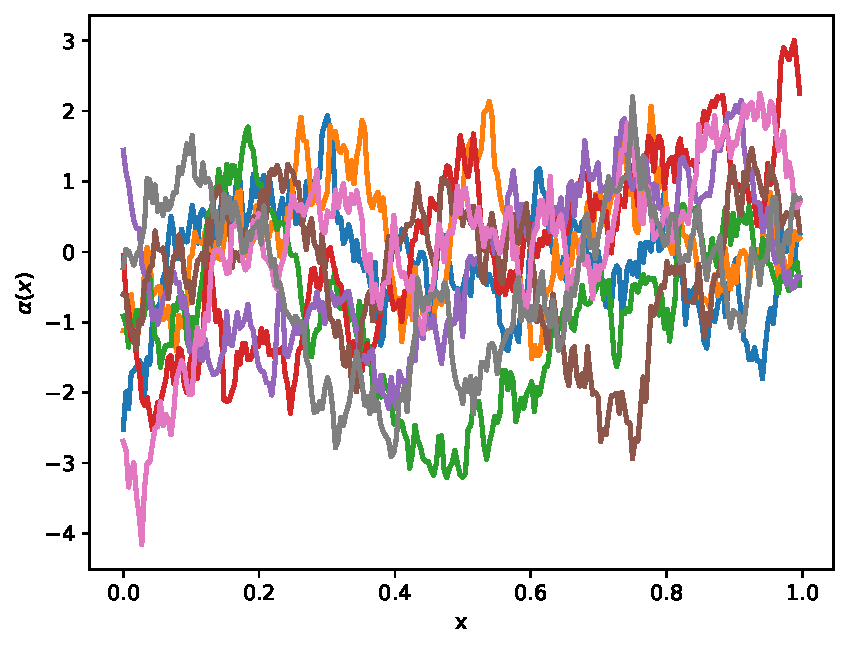
\includegraphics[width=0.45\linewidth]{figures/samples_nu0_5.pdf}
        \hfill
        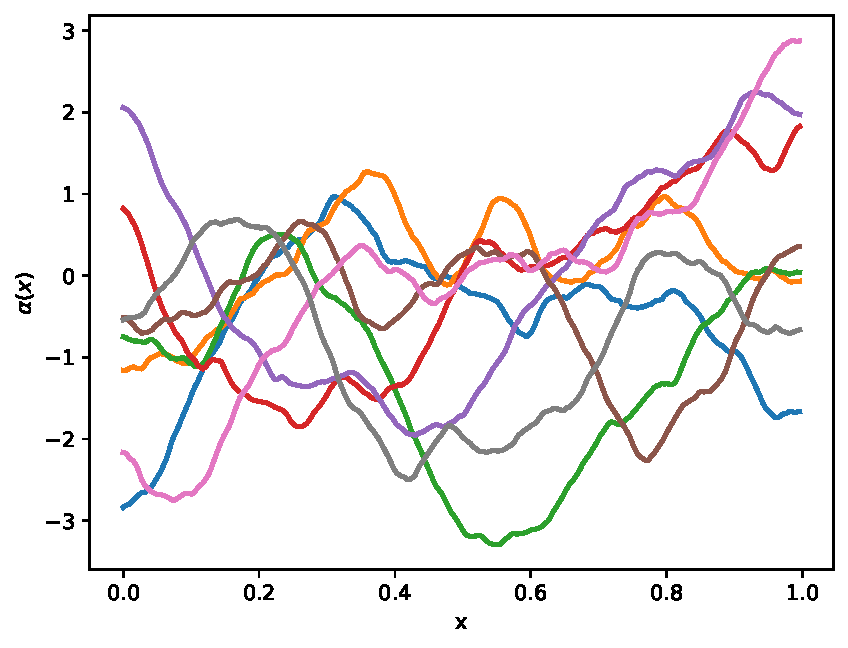
\includegraphics[width=0.45\linewidth]{figures/samples_nu1_5.pdf}
    \end{center}
    \caption{Random samples $\alpha(x)$ drawn from $\pi^{(h)}(\cdot|\nu,\kappa)$ for $a=1$, $\nu=\frac{1}{2}$ (left) and $a=2$, $\nu=\frac{3}{2}$ (right). In both cases the correlation length is $\kappa^{-1}=0.1$ and the number of gridcells is $N=256$. The samples are scaled by $\sigma^{-1}$ to make their variance $\sim 1$.}
    \label{fig:random_samples}
\end{figure}
Fig.~\ref{fig:random_samples} showns some random samples generates in this way for both $a=1$, $\nu=\frac{1}{2}$ and $a=2$, $\nu=\frac{3}{2}$.
\begin{figure}
    \begin{center}
        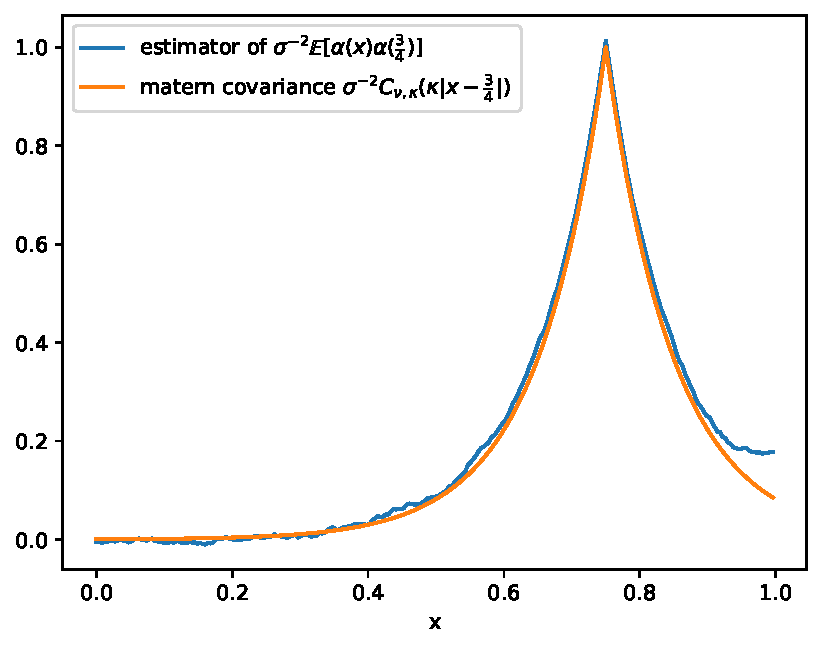
\includegraphics[width=0.45\linewidth]{figures/covariance_nu0_5.pdf}
        \hfill
        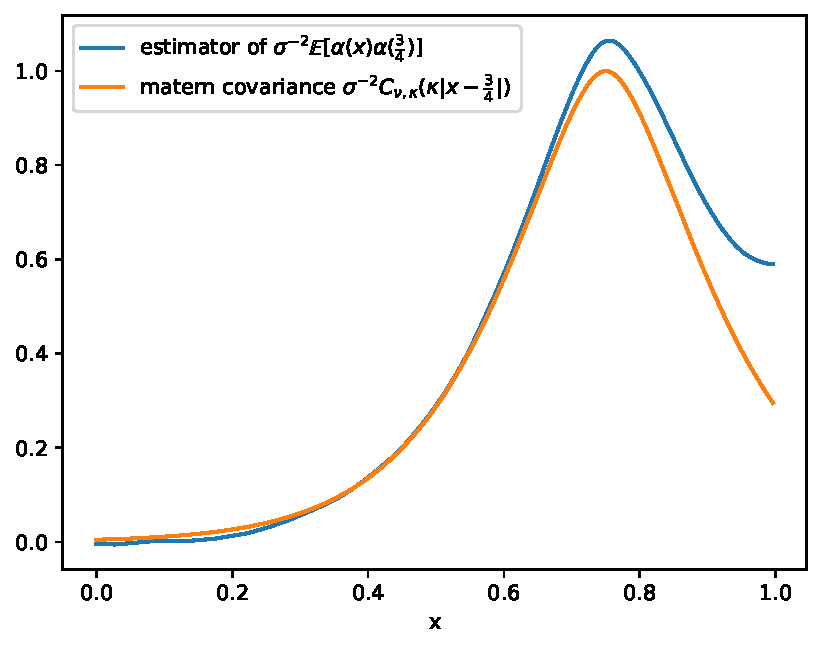
\includegraphics[width=0.45\linewidth]{figures/covariance_nu1_5.pdf}
    \end{center}
    \caption{Empirical covariance between the points $x$ and $y=\frac{3}{4}$ and Matern covariance function. Results are shown for $a=1$, $\nu=\frac{1}{2}$ (left) and $a=2$, $\nu=\frac{3}{2}$ (right). In both cases the correlation length is $\kappa^{-1}=0.1$ and the number of gridcells is $N=256$. The samples are scaled by $\sigma^{-1}$ to make their variance $\sim 1$.}
    \label{fig:lognormal_covariance}
\end{figure}
The corresponding covariance between $a$ and $y=\frac{3}{4}$ is visualised in Fig.~\ref{fig:lognormal_covariance} where we show both an estimator for the covariance on the interval $\Omega=[0,1]$ and the Matern covariance function. The two functins differ since von Neumann boundary conditions have been imposed to generate the samples.
\bibliographystyle{unsrt}
\bibliography{problem_description}
\end{document}